% -------------------------------------------------

\chapter{Examples}

\section{Toy Example Shallow Seismics: Inversion of Viscoelastic Observations}
You can find the input files for the small toy example in the directory \texttt{par/in\_and\_out/toy\_example}. To run the example you can use the shell script \texttt{run\_toy\_example.sh} in the directory \texttt{par}. It is adjusted for a PC with at least 4 CPUs. If you have less CPUs you have to adjust the number of processors in the input files as well as in the call of IFOS2D in the shell script. The shell script includes all relevant steps. First all libraries and IFOS2D are compiled. (Do not get nervous about the huge output during compiling.) If you run into problems during this step you maybe have to adjust the variables in \texttt{Makefile\_var} in the directory \texttt{contrib}. Afterwards IFOS2D starts to simulate observed data for the inversion. The simulated seismograms are renamed for the inversion and IFOS2D is again compiled with another model function which creates the initial models for the inverison on the fly (see section~\ref{gen_of_mod}). The last step in the shell script is the call of IFOS2D to start the inversion.\\

The true model used for the simulation of the observed data is shown in Figure~\ref{Rheinstetten_true_model} whereat the shot positions are marked by the red stars and the CPML frame is marked by the black dashed line. We consider a viscoelastic medium in this test and approximate a constant quality factor of $Q_s=Q_p=20$ in the analyzed frequency band up to 70\,Hz with three relaxation mechanisms of a generalized standard linear solid. The 36 two component receivers used in the inversion are located equidistantly between the sources with a receiver spacing of 1\,m.\\

In the inversion we only inverted for the shear wave velocity model. The initial model is a linear gradient and is shown in Figure~\ref{Rheinstetten_initial_vs_model}.  For the P wave velocity model as well as for the density model the true models (see Figure~\ref{Rheinstetten_true_model}\subref{true-vp-model-Rheinstetten} and \subref{true-rho-model-Rheinstetten}) are used. Furthermore, we use the correct rheological model.\\

You will need less than 1~GB working memory to run the inversion and approximately 250\,MB of data are written to hard disk. Normally 137~iteration steps are calculated and the inversion will take approximately 6 hours. The inversion results for the shear wave velocity are shown in Figure~\ref{Rheinstetten_inversion_result}. Figure~\ref{Rheinstetten_inversion_result}\subref{inv-vs-model-Rheinstetten} shows an image plot and Figure~\ref{Rheinstetten_inversion_result}\subref{vertical-vel-profiles-Rheinstetten} shows vertical velocity profiles through the shear wave velocity models (thick grey line: true model; black dashed line: initial model; blue line: inverted model at $x=20$\,m; red dashed line: inverted model at $x=25$\,m).\\

You can use the script \texttt{mfiles/Plot\_results\_toy\_example.m} to visualize the results of the toy example. This script can be used with Matlab or Octave.

\begin{figure}[ht]
\centering
\subfloat[][]{%
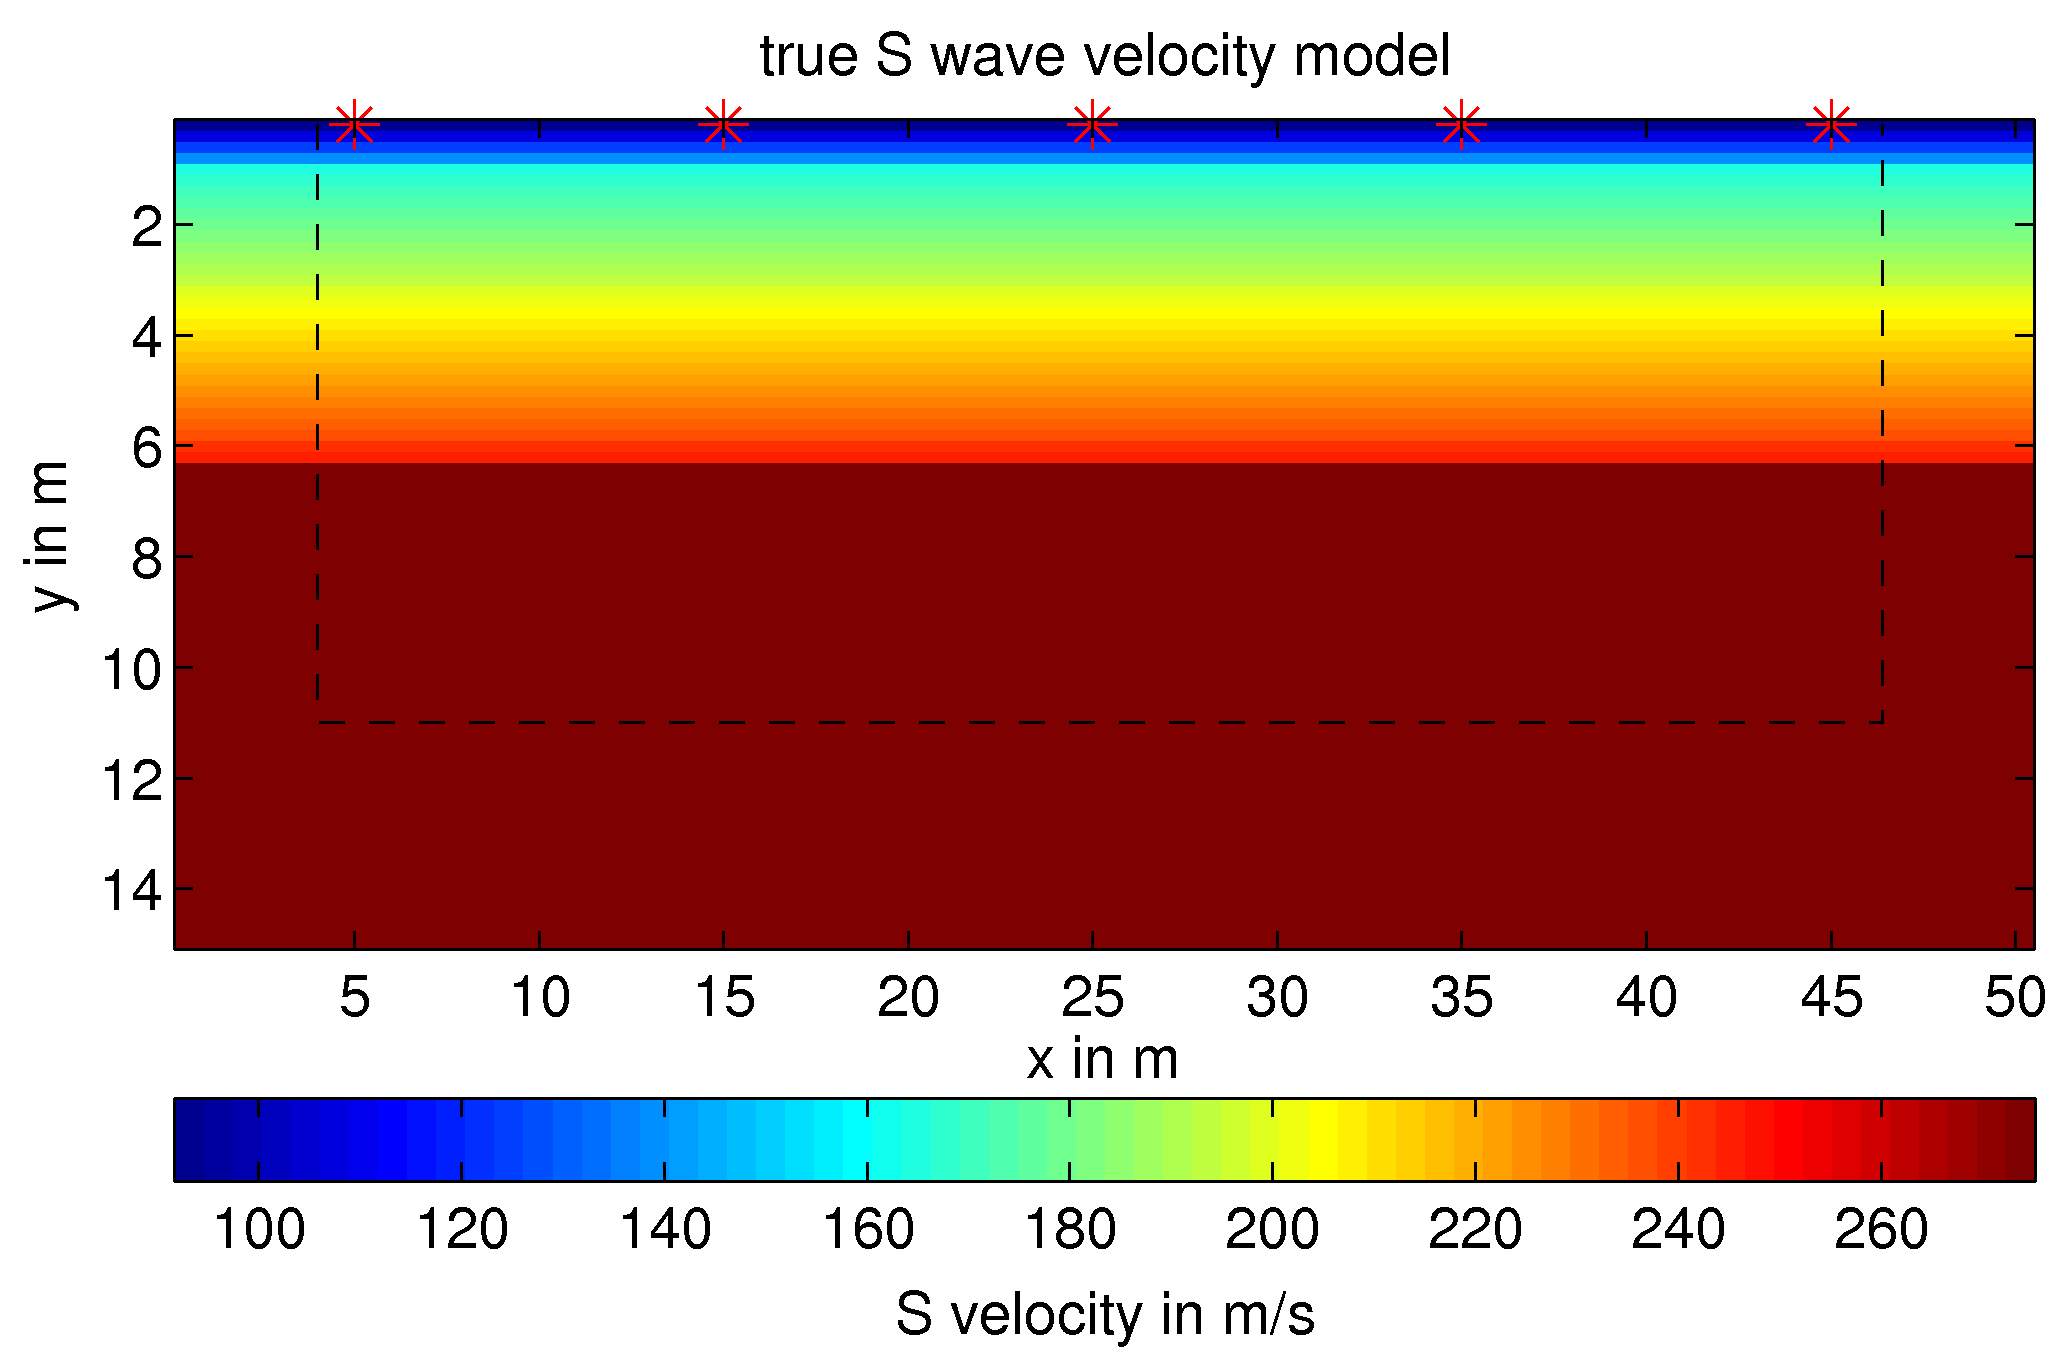
\includegraphics[width=10cm]{figures/Rheinstetten/true_vs_model}%
\label{true-vs-model-Rheinstetten}}\\%
\subfloat[][]{%
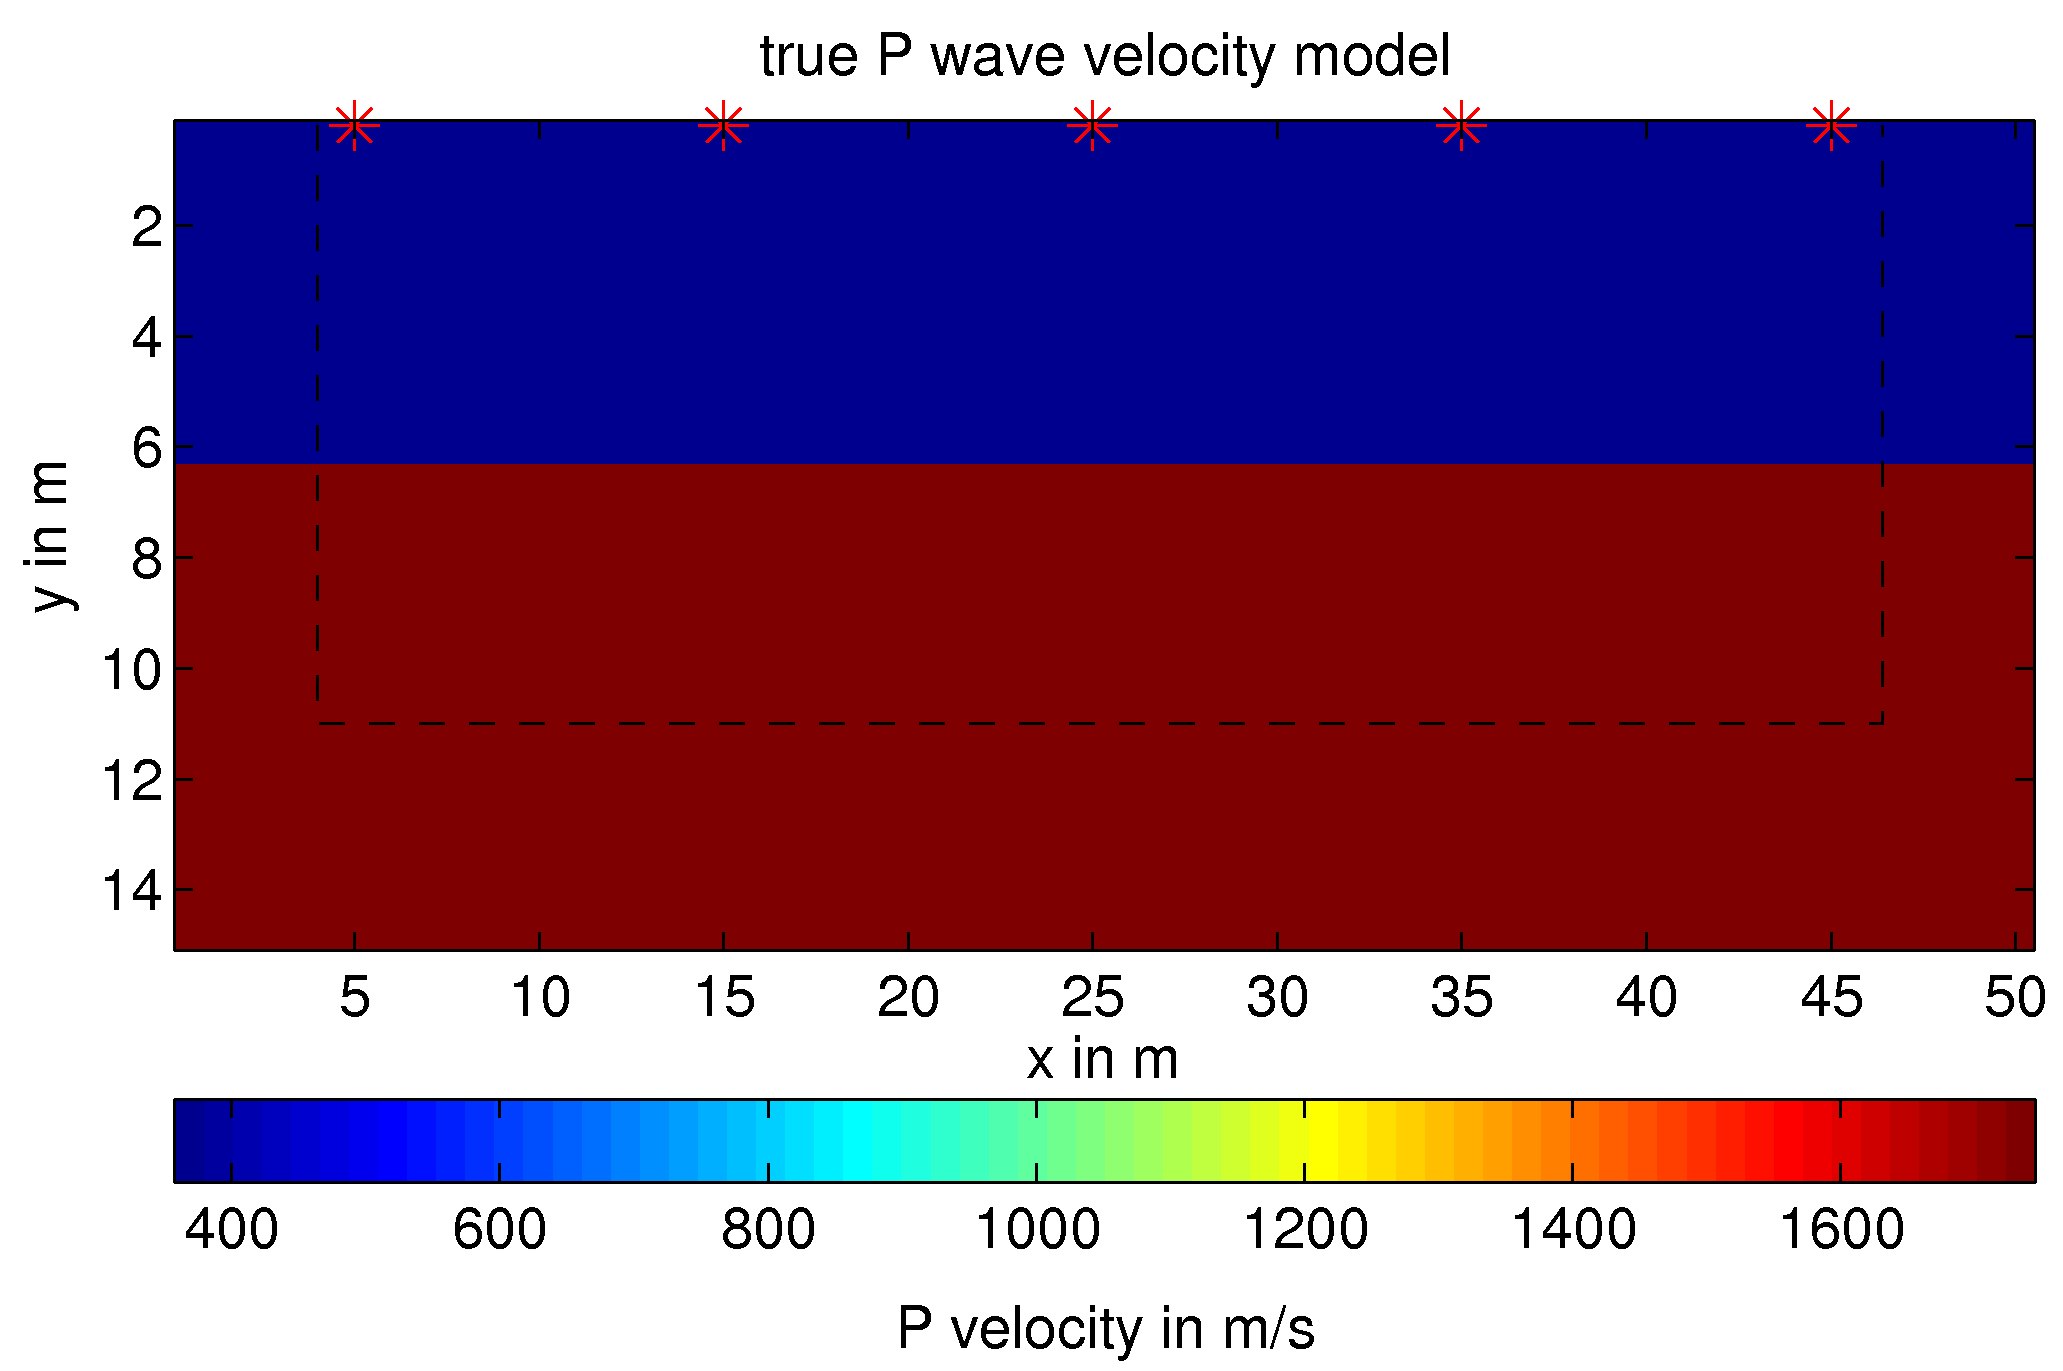
\includegraphics[width=10cm]{figures/Rheinstetten/true_vp_model}%
\label{true-vp-model-Rheinstetten}}\\%
\subfloat[][]{%
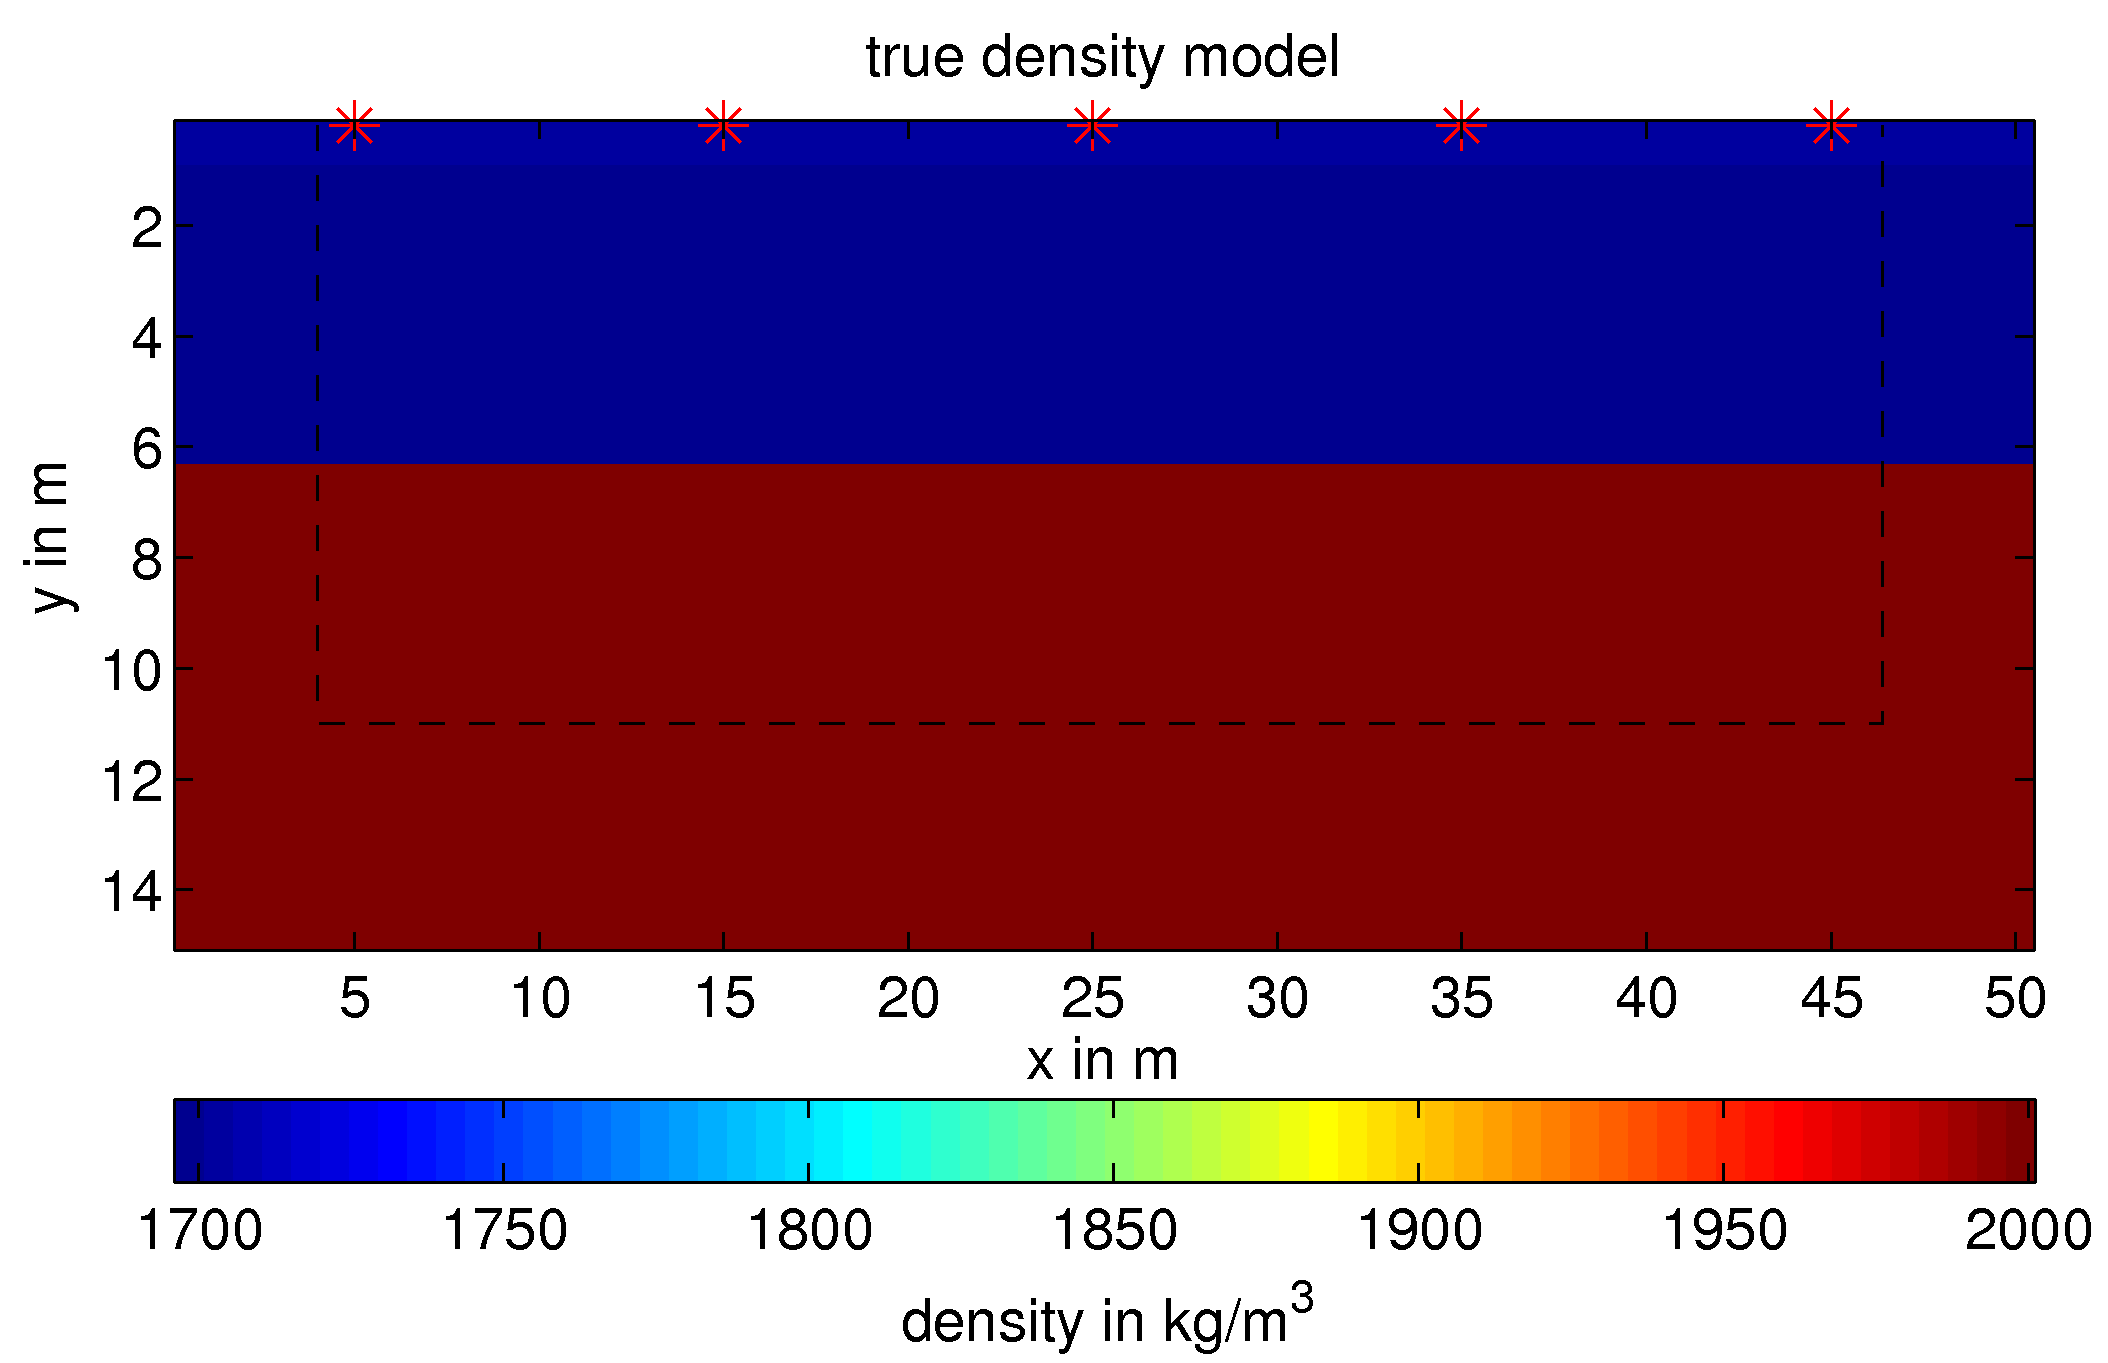
\includegraphics[width=10cm]{figures/Rheinstetten/true_rho_model}%
\label{true-rho-model-Rheinstetten}}
\caption{True models for \protect\subref{true-vs-model-Rheinstetten} the S wave velocity, \protect\subref{true-vp-model-Rheinstetten} the P wave velocity and \protect\subref{true-rho-model-Rheinstetten} the density used for the calculation of observed data. The red stars mark the five shots used in the inversion. The CPML frame is marked by the black dashed line.}
\label{Rheinstetten_true_model}
\end{figure}

\begin{figure}[ht]
\centering
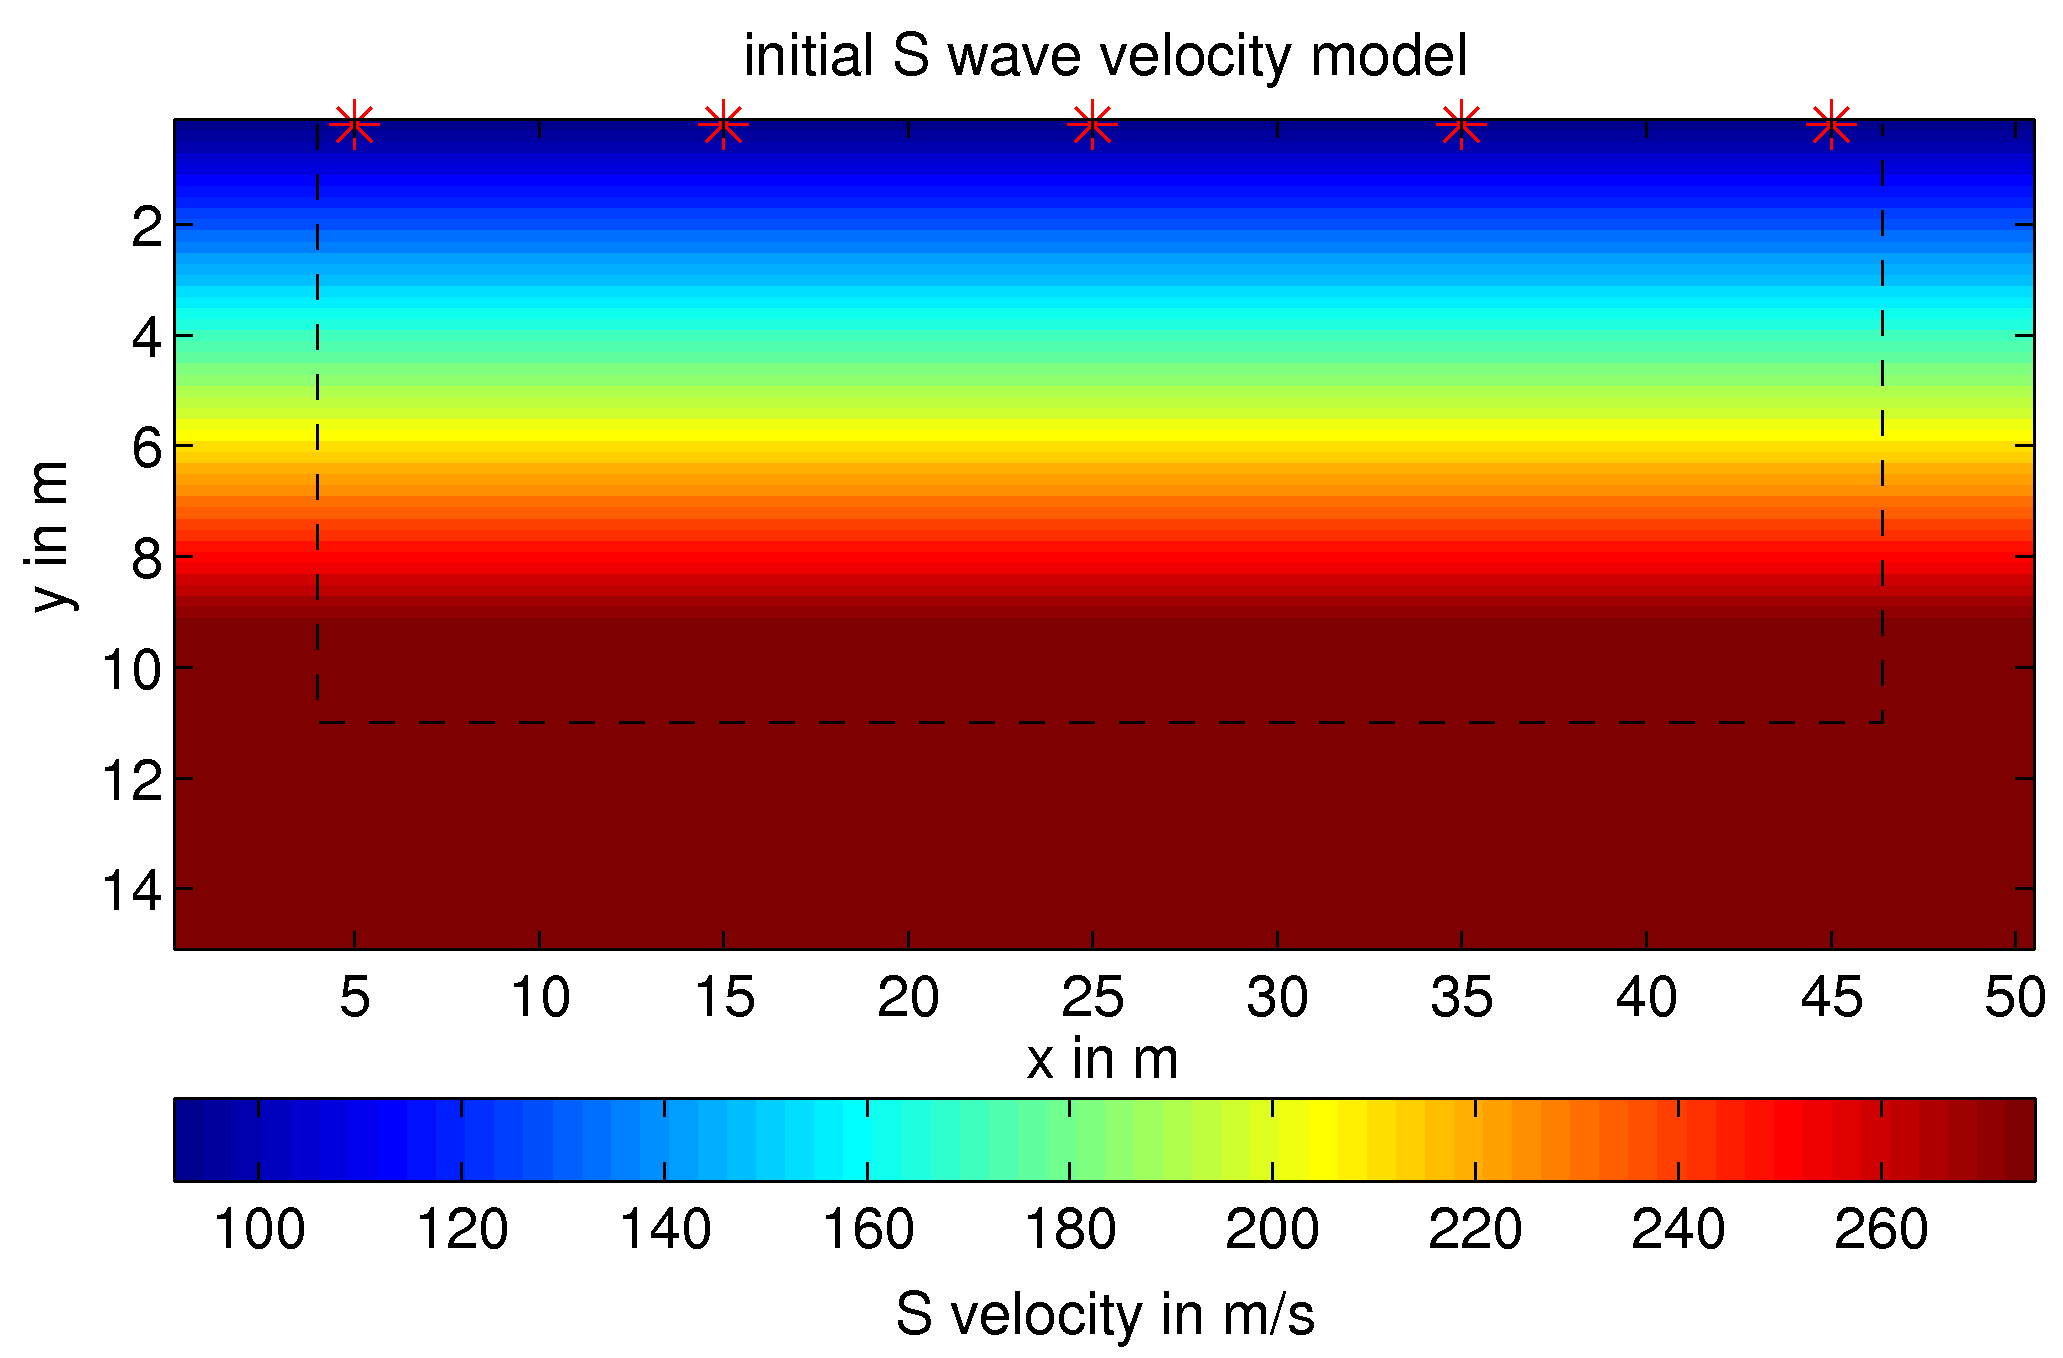
\includegraphics[width=10cm]{figures/Rheinstetten/start_vs_model}
\caption{Initial shear wave velocity model. The red stars mark the five shots used in the inversion. The CPML frame is marked by the black dashed line.}
\label{Rheinstetten_initial_vs_model}
\end{figure}

\begin{figure}[ht]
\centering
\subfloat[][]{%
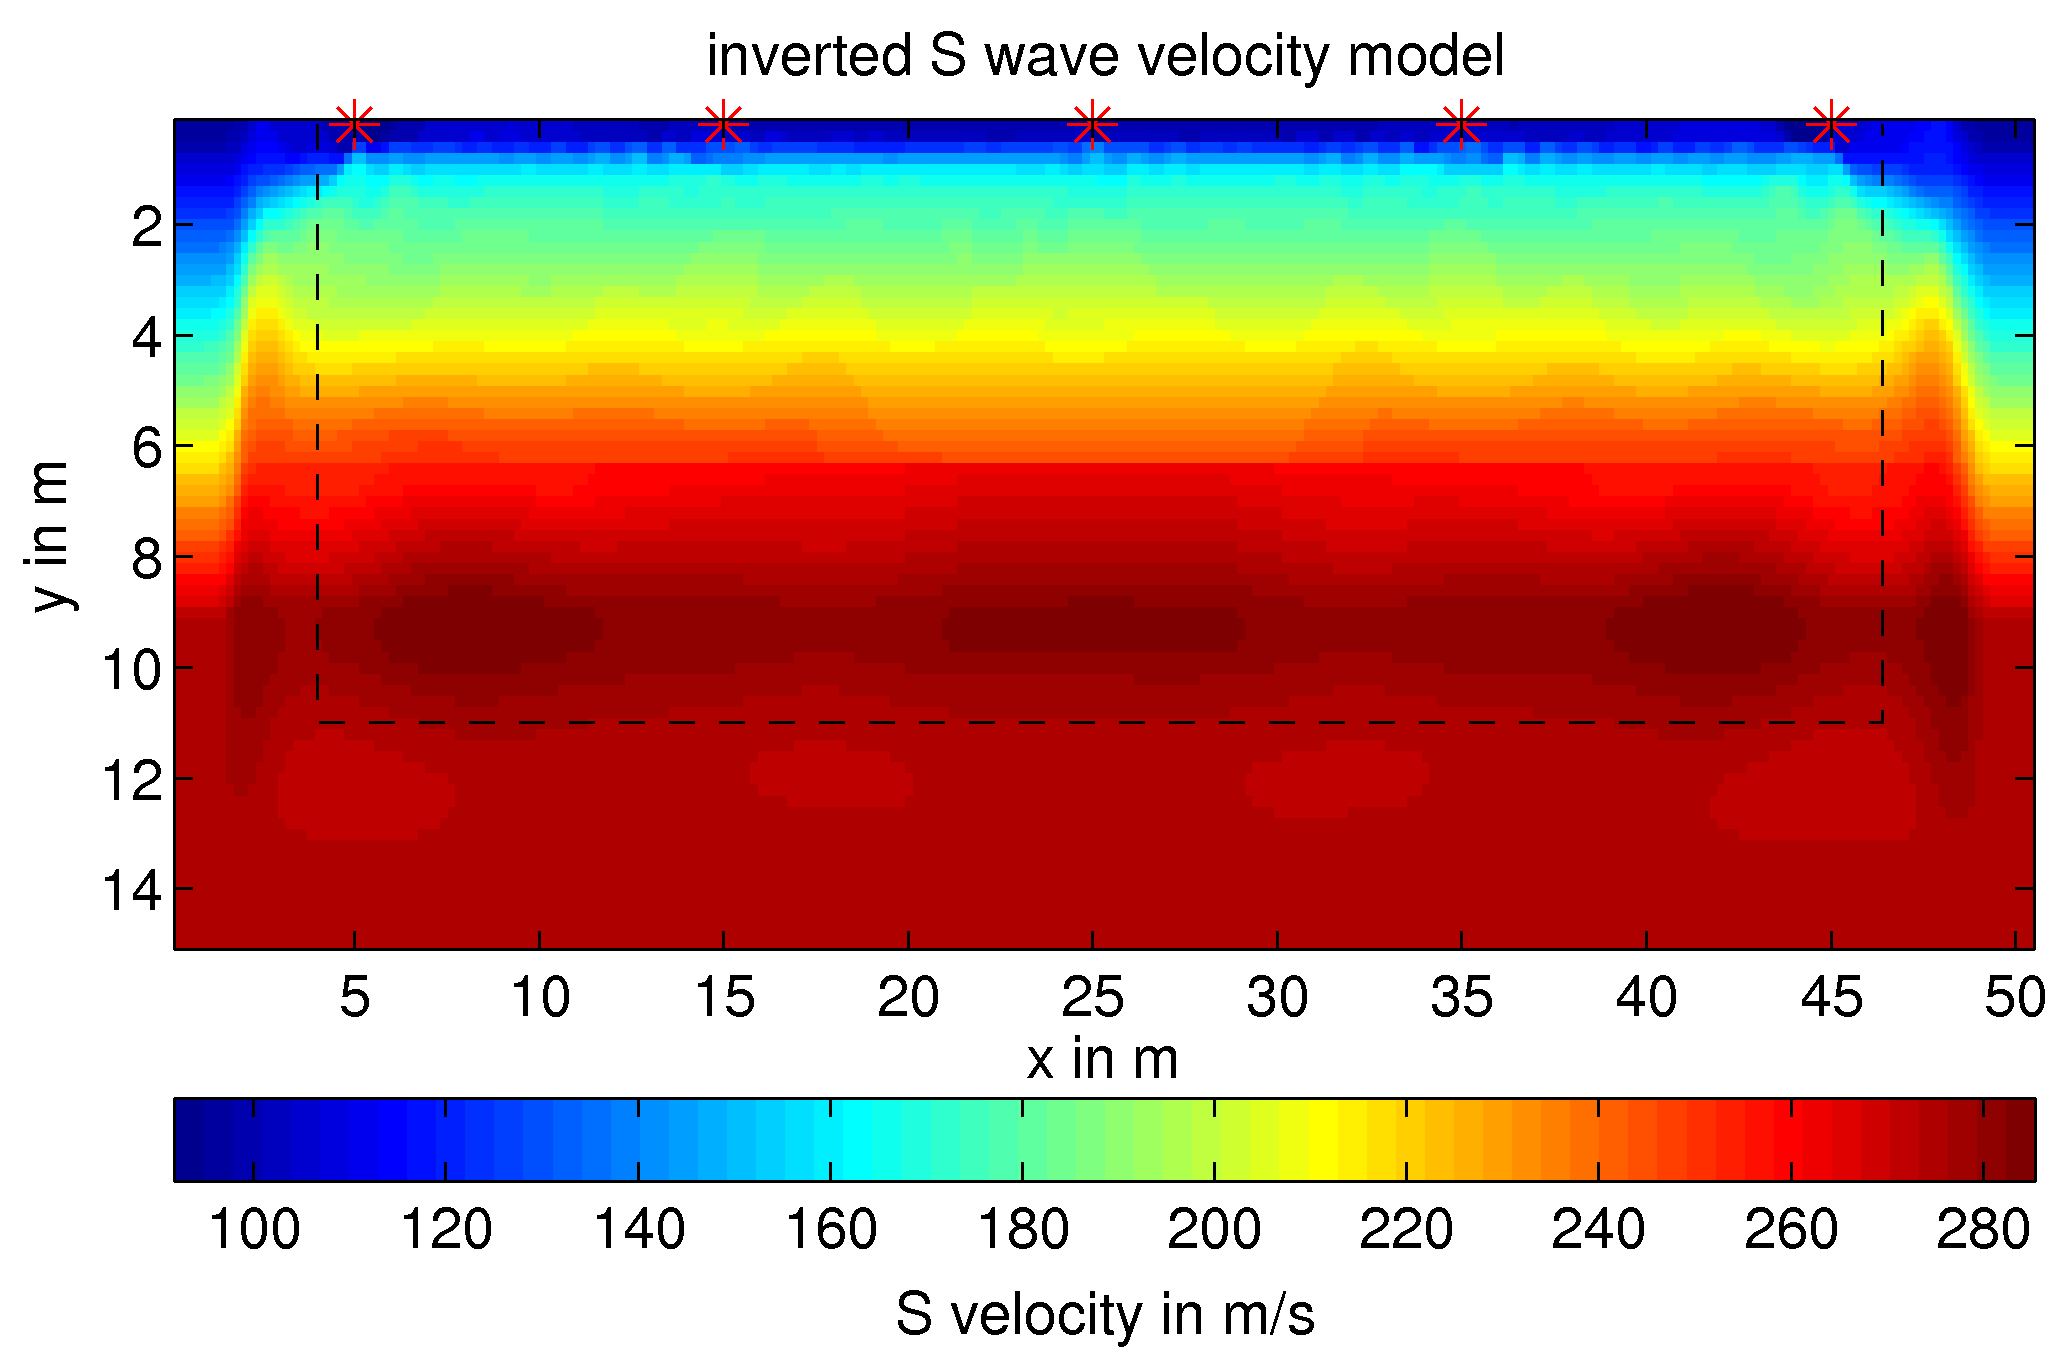
\includegraphics[width=10cm]{figures/Rheinstetten/inv_vs_model}%
\label{inv-vs-model-Rheinstetten}}%
\hspace{0.2 cm}
\subfloat[][]{%
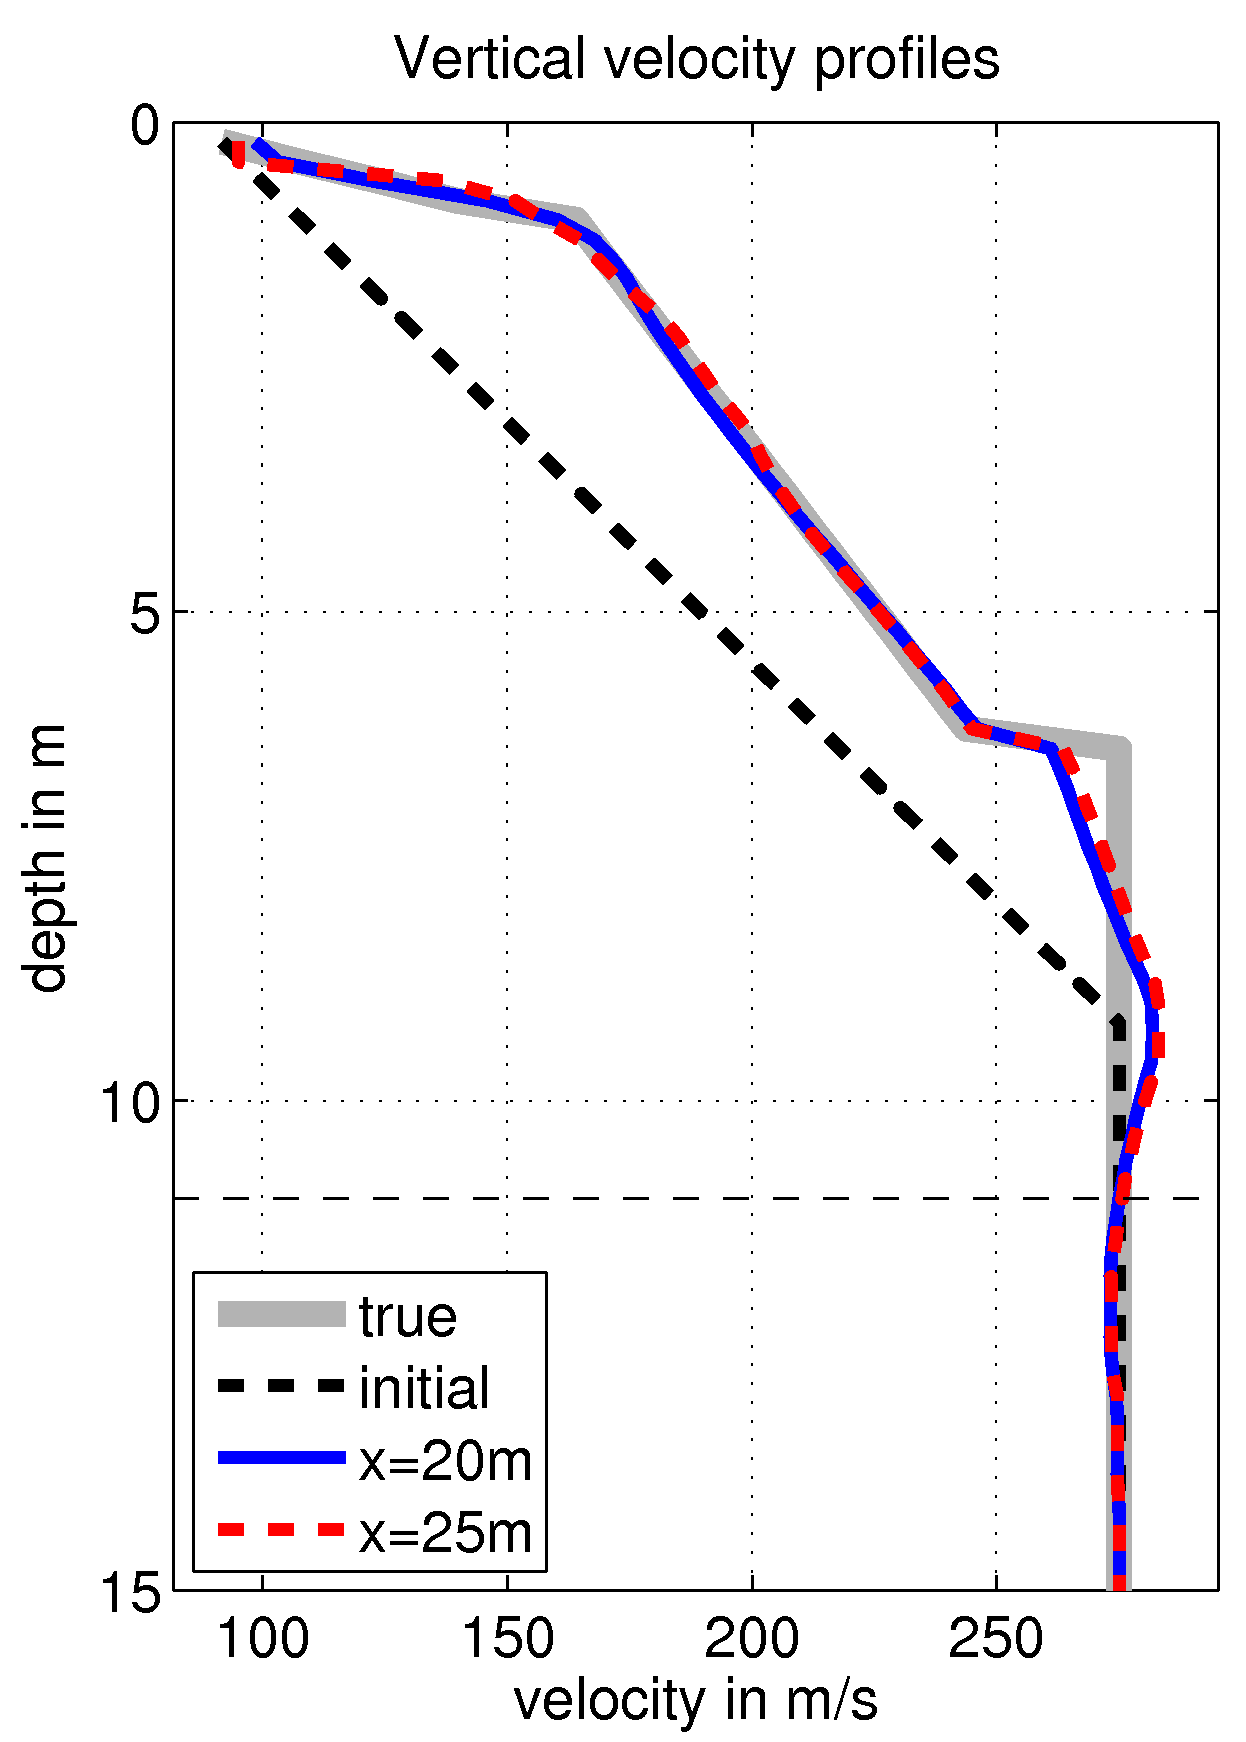
\includegraphics[width=5cm]{figures/Rheinstetten/vertical_vel_profiles}%
\label{vertical-vel-profiles-Rheinstetten}}
\caption{Inverted shear wave velocity model. \protect\subref{inv-vs-model-Rheinstetten} shows an imageplot of the inversion result. The red stars mark the source positions and the black dashed line marks the CPML frame. \protect\subref{vertical-vel-profiles-Rheinstetten} shows vertical velocity profiles of the shear wave velocity models. The true model is plotted with the thick grey line, the initial velocity model is represented by the dashed black line and two vertical profiles at $x$=20\,m and $x$=25\,m of the inverted model are plotted in red and blue. The CPML frame is again marked by the thin black line at 11\,m depth.}
\label{Rheinstetten_inversion_result}
\end{figure}

\clearpage
